\documentclass{amsart}
\usepackage[margin=3cm]{geometry}                % See geometry.pdf to learn the layout optons. There are lots.
\geometry{letterpaper}                   % ... or a4paper or a5paper or ...
%\geometry{landscape}                % Activate for for rotated page geometry
\usepackage[parfill]{parskip}    % Activate to begin paragraphs with an empty line rather than an indent
\usepackage{float}
\usepackage{graphicx}
\usepackage{amssymb}
\usepackage{epstopdf}
\usepackage{siunitx}
\usepackage{subcaption}

\DeclareGraphicsRule{.tif}{png}{.png}{`convert #1 `dirname #1`/`basename #1 .tif`.png}

\title{Lab 7: Lenses}
\author{Caspar \textsc{Lant}} % Author name

\date{\today} % Date for the report

\begin{document}

\bigskip

\maketitle % Insert the title, author and date
\begin{center}

Intermediate Experimental Physics I\\
\vspace{1.5cm}
\begin{tabular}{|l r|}
\hline
Section: & 002\\
&\\
Date Performed: & November 6, 2015 \\ % Date the experiment was performed
Date Due: & November 13, 2015\\
&\\
Partner: & Sam P. Meier \\ % Partner names
Professor: & Prof. Andrew Kent\\
Instructor: & David Mykytyn\\ % Instructor/supervisor
\hline
\end{tabular}
\end{center}
\vspace{50mm}
\pagebreak

\paragraph{\textbf{The Objective} of this week's experiment was to put our vast theoretical knowledge of lenses to application. It is always a remarkable thing to see what was once pure abstraction validated though rigorous scientific experimentation. }
\section{Theoretical Background/ Abstract}
\paragraph{Lenses have been of interest to us humans for a long time now. Convex lenses, concave lenses, even planar mirrors have all been the subjects of frenzied study through the ages. This should come as no surprise, given how fantastically useful they are to creatures who experience the world, mainly, through sight. We are mainly interested in what happens to the light from objects in front of the lense }
\begin{equation}
\frac{1}{s_i}+ \frac{1}{s_o} = \frac{1}{f}
\end{equation}
\begin{equation}
\frac{1}{f} = (n-1)\Big(\frac{1}{R_1} - \frac{1}{R_2}\Big)
\end{equation}

\medskip
\subsection{Concave Lenses \nopunct} are lenses who's with is minimum at their center point. Then focal length of a convex lens is negative, by convention. Concave lenses are usually classified as "divergent" lenses, and produce virtual images on the same side as the object.
\begin{center}
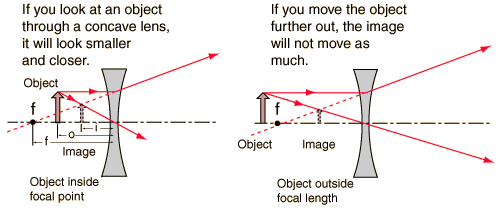
\includegraphics[width = 4in]{ccv.png}
\end{center}

\subsection{Convex Lenses \nopunct} are lenses who's width is maximal at their center point. The focal length of a convex lens is positive, by convention. Convex lenses are capable of producing both real and virtual images, depending on where the object is in relation to the lens' focal point. Objects placed between the focal point and the lens will produce an upright, virtual image of greater size. Objects farther away from the lens than its focal point will produce real and inverted images, as shown in the following figure:
\begin{center}
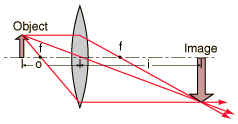
\includegraphics[width = 2.5in]{cvex1.png}
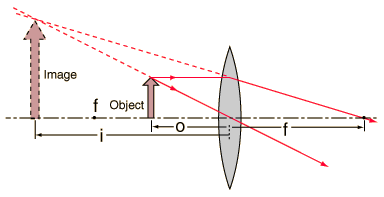
\includegraphics[width = 2.5in]{cvex2.png}
\end{center}

\subsection{Matrix Optics\nopunct \\}
{It is important to talk about another method of analyzing systems of lenses, which has the potential to make complex much simpler, as well as much harder. We know that lenses, as well as other optical objects, like mirrors, transform the angle and position of light rays in the parallel plane. Because light rays are easily represented as vectors, it makes sense to characterize each lens in a given system with a matrix, like the ones seen in the table below:}

\begin{table}[H]
\centering
\label{my-label}
\begin{tabular}{llll}
\multicolumn{1}{c}{Curved Refraction}                                                           & \multicolumn{1}{c}{Free Space}                                & \multicolumn{1}{c}{Thin Lens}                                        &  \\
$\left[\begin{array}{cc}1 & 0 \\- \frac{n_1-n_2}{R \ n_2} & \frac{n_1}{n_2}\end{array}\right]$ & $\left[\begin{array}{cc}1 & d \\0 & 1\end{array}\right]$ & $\left[\begin{array}{cc}1 & 0 \\- \frac{1}{f} & 1\end{array}\right]$ &
\end{tabular}
\end{table}

\paragraph{The thin lens matrix in the above table is a composition of a curved refraction matrix, a free space matrix, and another curved refraction matrix. The assumption for thin lenses is that the focal length of the lens far exceeds its width, and the distance travelled by a ray of light inside the lens can be discounted.}

\section{Experimental Procedure}
\begin{enumerate}
\item Begin by placing the laser apparatus on the steel bar supplied by your teaching assistant. Turn it on.
\item Place a diffuser (or a Wratten Filter) in the path of the laser, some millimeters away
\item Place a screen at the opposite end of the optical bench
\item Place each convex, convergent lens some distance between the laser and the opposing screen.
\item Minimize the diameter of the laser's 'spot' on the screen to determine the lens' focal length. The distance between the lens and the screen is the magnitude of the lens' focus.
\item Repeat steps 4 and 5 for each concave, divergent lens, with the following addition to procedure:
\item Once you are confident that you have found the lens' focus, shift the lens in the plane perpendicular to the incident light rays. The spot on the screen should move by the same amount. If it does not, you are not at the focus.
\item Place the lens with a focal length of  +48mm in the path of the laser. Change the position of this lens several times, and move the screen such that the image (spot) is in focus.  Measure the object and image distances and calculate the focal length in each case to verify the lens equation above.
\item This time, place two lenses in the path of the laser. These lenses should have focal lengths +127mm and +252mm, and should share the same frame. Measure the focal length of this pair and compare this to a result you came up with mathematically.
\item Separate the two lenses by a distance of 15 cm (you'll need an additional mount for this) and place the closes lens 15cm away from the arrow object
\item Create a simple telescope with two lenses
\item Extra Credit: create a simple telescope with three lenses
\end{enumerate}

\section{Two Separated Lenses}

\begin{figure}[H]
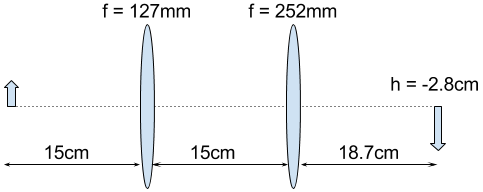
\includegraphics[width=0.49\textwidth]{ConvexLensSystem.png}
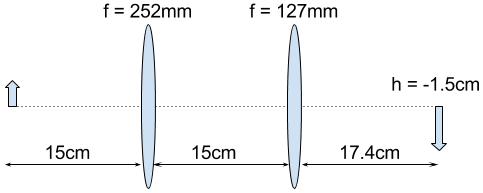
\includegraphics[width=0.49\textwidth]{ConvexLensSystem(1).png}
\end{figure}

\begin{figure}[h]
\centering
\caption{Systems of Convex Lenses that Produce Real Inverted Images:}
\end{figure}

\medskip

\begin{figure}[H]
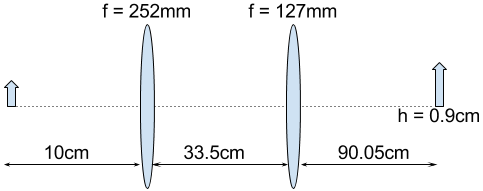
\includegraphics[width=0.49\textwidth]{ConvexLensSystem(2).png}
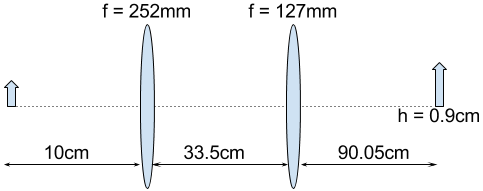
\includegraphics[width=0.49\textwidth]{ConvexLensSystem(2).png}
\end{figure}

 \begin{figure}[H]
\centering
\caption{Systems of Convex Lenses that Produce Real Upright Images:}
\end{figure}

\medskip

\section{Simple Telescope}
\begin{figure}[h]
\centering
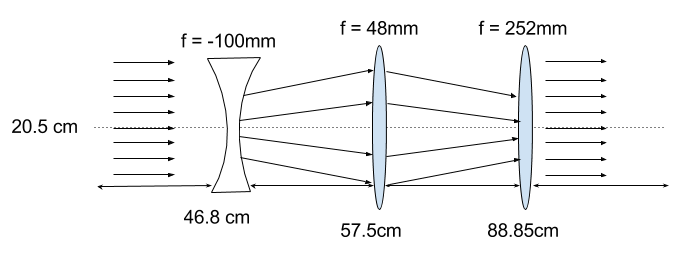
\includegraphics[width = 14cm]{SimpleTelescope.png}
\caption{Extra Credit: Three Lens Simple Telescope}
\end{figure}

\pagebreak

\section{Tables and Analysis}
\begin{table}[H]
\centering
\caption{Experimental Values for Image Distance and Height}
\label{my-label}
\begin{tabular}{c|c|c|c|c|c|c}
$f_1$ (mm) & $f_2$ (mm) & $h_o$ (mm) & $h_i$ (mm) & $s_{1_o}$ (mm) & $s_{1_i}$ (mm) & $s_{2_o}$ (mm) \\ \hline
127.0        & 252.0        & 10.0         & -28.0        & 150.0       & 150.0   & 187.0       \\
252.0        & 127.0        & 10.0         & -15.0        & 150.0       & 150.0   & 174.0       \\
252.0        & 127.0        & 10.0         & 9.0          & 100.0       & 335.0   & 900.5
\end{tabular}
\end{table}

\begin{table}[H]
\centering
\caption{Experimental and Theoretical Values for Focal Length and Height}
\label{my-label}
\begin{tabular}{c|c|c||c|c}
$\frac{1}{f\prime}$ (mm) & $\frac{1}{s_o} + \frac{1}{s_i}$ (mm) & \% Error & $s_o/s_i$ & ${h_o}/{h_i}$ \\ \hline
0.011842                 & 0.012014                             & 1.452    & 0.802             & -0.357            \\
0.011842                 & 0.012414                             & 4.826    & 0.862             & -0.667            \\
0.011842                 & 0.011110                             & 6.179    & 0.111             & 1.111
\end{tabular}
\end{table}

\section{Questions}

\begin{enumerate}
\item {\textit{If you were to use a green laser beam to measure the focal length, would you get the same value? Does your answer bear on chromatic aberration in which a white object is focused as a somewhat blurred color image?}
\begin{quote}
It is assumed that, because we are using a laser, the light incident on our object lenses is coherent and columnar?composed of parallel rays. Coherent light is that which is uniform in wavelength. Green light of uniform wavelength would give us a slightly different value for focal length, because angle of refraction depends somewhat on frequency. This discrepancy is overlooked, however, when we use the thin lens approximation. The only refraction that goes on in the systems we are working with occurs \textit{within} the lens, which we take to have width zero.
\end{quote}}

\item{\textit{If two lenses have exactly the same dimensions but have different indexes of refraction, will their focal lengths be the same? Discuss.}
\begin{quote}
The lensmaker's equation states that the focal length of a lens is proportional to its index of refraction, in the following way:
$$ \frac{1}{f} = \dfrac{n_{lens} - n_0}{n_0}\left(\frac{1}{R_1} - \frac{1}{R_2}\right) $$
\end{quote}}

\item{\textit{Using Eq.(1) twice, prove Eq.(4).}
\begin{quote}

%\begin{equation}
%\frac{1}{s_i}+ \frac{1}{s_o} = \frac{1}{f} \rightarrow \frac{1}{f_1}+ \frac{1}{f_2} = \frac{1}{f \prime} ,\ \  \[\boxed{ s_{1_i} = - s_{2_o}}\]
%\end{equation}

$$\frac{1}{s_i}+ \frac{1}{s_o} = \frac{1}{f} \rightarrow \frac{1}{f_1}+ \frac{1}{f_2} = \frac{1}{f \prime} , \ \ s_{1_i} = - s_{2_o} $$
$$ \frac{1}{f_1}+ \frac{1}{f_2} = \left(\frac{1}{s_{1_i}}+ \frac{1}{s_{1_o}}\right) + \left(\frac{1}{s_{2_i}}+ \frac{1}{s_{2_o}} \right) \rightarrow  \left(\frac{1}{s_{2_o}} -  \frac{1}{s_{2_o}}\right) +  \frac{1}{s_{1_o}} +  \frac{1}{s_{2_i}} =  \frac{1}{s_{1_o}} +  \frac{1}{s_{2_i}}$$

\[ \boxed{
$$ \frac{1}{s_{1_o}} +  \frac{1}{s_{2_i}} = \frac{1}{f \prime}$$}
\]

\end{quote}}

\end{enumerate}

\section{Error Analysis}
\paragraph{Let's do some error analysis! Our uncertainty in measurement in length and height is given by the following formula, according to Taylor's book. The error bars on the focal length of each lens is said to be zero, as the manufacturer of the lens did not supply any measure of precision or manufacturing tolerance. }
\paragraph{}
\begin{figure}[H]
\begin{minipage}{.55\textwidth}
\begin{equation}
\large\delta \left[\dfrac{1}{s_o} + \dfrac{1}{s_i}\right] = \left|\dfrac{1}{s_o} + \dfrac{1}{s_i} \right| \sqrt{\left( \dfrac{\delta s_o}{s_o} \right)^2+ \left(\dfrac{\delta s_i}{s_i}\right)^2}
\end{equation}
\end{minipage}
%
\begin{minipage}{.4\textwidth}
\begin{table}[H]
\centering
\label{my-label}
\begin{tabular}{c|c|c}
$\delta$ & $\frac{1}{s_o} + \frac{1}{s_i} + \delta $         &   $\frac{1}{s_i} + \frac{1}{s_i} - \delta  $       \\ \hline
0.0005134          & 0.0125277 & 0.0115009 \\
0.0005463          & 0.0129601 & 0.0118675 \\
0.0005589          & 0.0116694 & 0.0105516
\end{tabular}
\end{table}
\end{minipage}
\end{figure}
\paragraph{As you can see, our experimentally-derived values for the inverse of focal length of the lens system \\($\frac{1}{s_o} + \frac{1}{s_i}$) fall well within out error bounds. The only way I can imagine lowering our values for uncertainty are through the use of more-precise instruments of measurements. Additionally, it's possible that we accrued some error though by using imperfectly-shaped lenses. }




\end{document}
